% Graphic for TeX using PGF
% Title: /home/nevj/common/Dia/vdl2.dia
% Creator: Dia v0.97.3
% CreationDate: Thu Sep 27 20:35:12 2018
% For: nevj
% \usepackage{tikz}
% The following commands are not supported in PSTricks at present
% We define them conditionally, so when they are implemented,
% this pgf file will use them.
%\begin{document}
%\begin{landscape}
%\label{fig:vdl}
\begin{figure}[!h]
  \centering

\ifx\du\undefined
  \newlength{\du}
\fi
\setlength{\du}{15\unitlength}
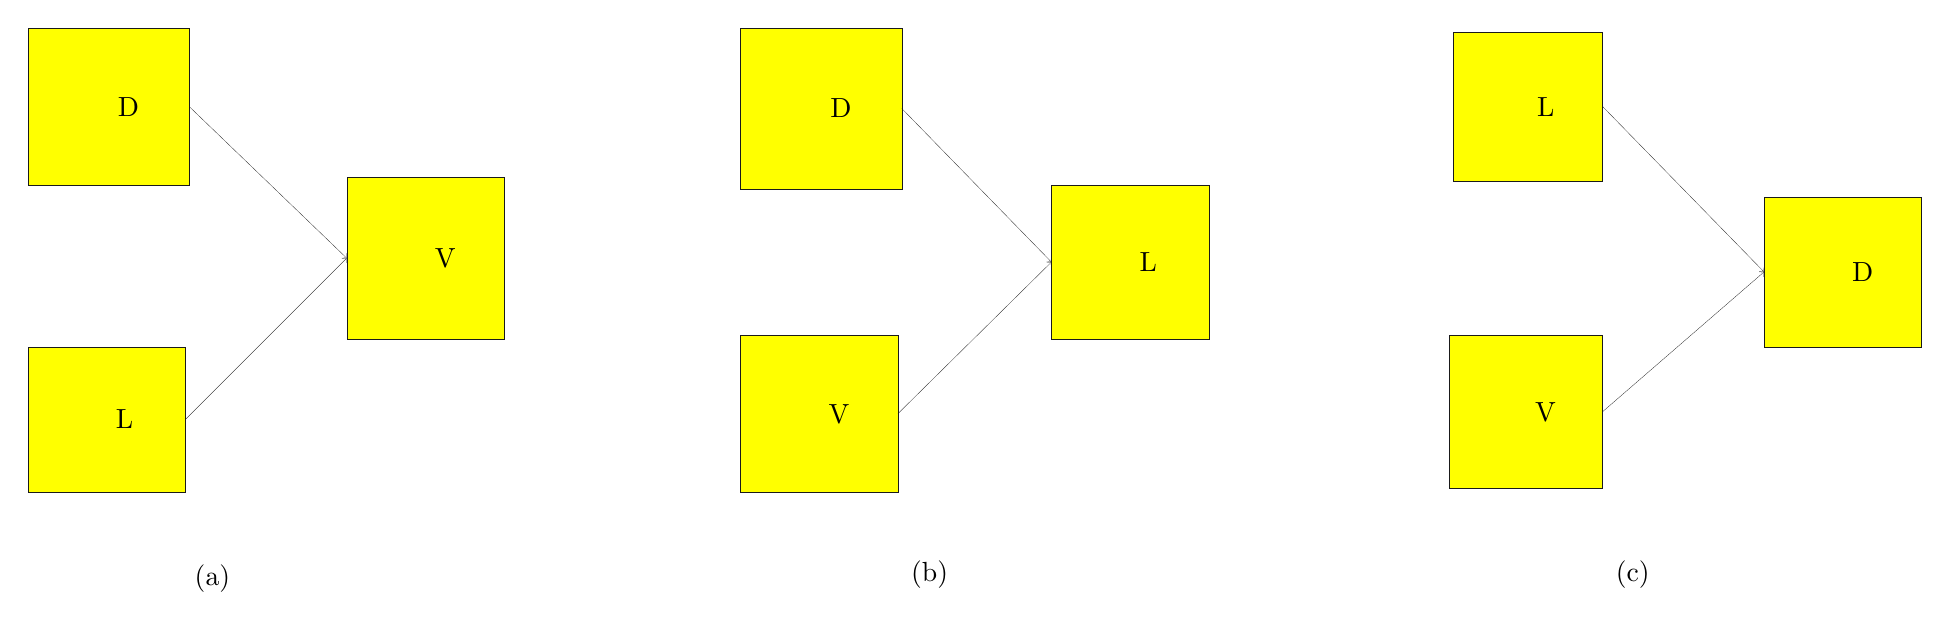
\begin{tikzpicture}
\pgftransformxscale{1.000000}
\pgftransformyscale{-1.000000}
\definecolor{dialinecolor}{rgb}{0.000000, 0.000000, 0.000000}
\pgfsetstrokecolor{dialinecolor}
\definecolor{dialinecolor}{rgb}{1.000000, 1.000000, 1.000000}
\pgfsetfillcolor{dialinecolor}
\pgfsetlinewidth{0.100000\du}
\pgfsetdash{}{0pt}
\pgfsetdash{}{0pt}
\pgfsetmiterjoin
\definecolor{dialinecolor}{rgb}{1.000000, 1.000000, 0.000000}
\pgfsetfillcolor{dialinecolor}
\fill (0.950000\du,1.050000\du)--(0.950000\du,3.050000\du)--(3.000000\du,3.050000\du)--(3.000000\du,1.050000\du)--cycle;
\definecolor{dialinecolor}{rgb}{0.101961, 0.101961, 0.101961}
\pgfsetstrokecolor{dialinecolor}
\draw (0.950000\du,1.050000\du)--(0.950000\du,3.050000\du)--(3.000000\du,3.050000\du)--(3.000000\du,1.050000\du)--cycle;
\pgfsetlinewidth{0.100000\du}
\pgfsetdash{}{0pt}
\pgfsetdash{}{0pt}
\pgfsetmiterjoin
\definecolor{dialinecolor}{rgb}{1.000000, 1.000000, 0.000000}
\pgfsetfillcolor{dialinecolor}
\fill (0.950000\du,5.100000\du)--(0.950000\du,6.950000\du)--(2.950000\du,6.950000\du)--(2.950000\du,5.100000\du)--cycle;
\definecolor{dialinecolor}{rgb}{0.101961, 0.101961, 0.101961}
\pgfsetstrokecolor{dialinecolor}
\draw (0.950000\du,5.100000\du)--(0.950000\du,6.950000\du)--(2.950000\du,6.950000\du)--(2.950000\du,5.100000\du)--cycle;
\pgfsetlinewidth{0.100000\du}
\pgfsetdash{}{0pt}
\pgfsetdash{}{0pt}
\pgfsetmiterjoin
\definecolor{dialinecolor}{rgb}{1.000000, 1.000000, 0.000000}
\pgfsetfillcolor{dialinecolor}
\fill (5.000000\du,2.950000\du)--(5.000000\du,5.000000\du)--(7.000000\du,5.000000\du)--(7.000000\du,2.950000\du)--cycle;
\definecolor{dialinecolor}{rgb}{0.101961, 0.101961, 0.101961}
\pgfsetstrokecolor{dialinecolor}
\draw (5.000000\du,2.950000\du)--(5.000000\du,5.000000\du)--(7.000000\du,5.000000\du)--(7.000000\du,2.950000\du)--cycle;
\pgfsetlinewidth{0.100000\du}
\pgfsetdash{}{0pt}
\pgfsetdash{}{0pt}
\pgfsetmiterjoin
\definecolor{dialinecolor}{rgb}{1.000000, 1.000000, 0.000000}
\pgfsetfillcolor{dialinecolor}
\fill (10.000000\du,1.050000\du)--(10.000000\du,3.100000\du)--(12.050000\du,3.100000\du)--(12.050000\du,1.050000\du)--cycle;
\definecolor{dialinecolor}{rgb}{0.101961, 0.101961, 0.101961}
\pgfsetstrokecolor{dialinecolor}
\draw (10.000000\du,1.050000\du)--(10.000000\du,3.100000\du)--(12.050000\du,3.100000\du)--(12.050000\du,1.050000\du)--cycle;
\pgfsetlinewidth{0.100000\du}
\pgfsetdash{}{0pt}
\pgfsetdash{}{0pt}
\pgfsetmiterjoin
\definecolor{dialinecolor}{rgb}{1.000000, 1.000000, 0.000000}
\pgfsetfillcolor{dialinecolor}
\fill (10.000000\du,4.950000\du)--(10.000000\du,6.950000\du)--(12.000000\du,6.950000\du)--(12.000000\du,4.950000\du)--cycle;
\definecolor{dialinecolor}{rgb}{0.101961, 0.101961, 0.101961}
\pgfsetstrokecolor{dialinecolor}
\draw (10.000000\du,4.950000\du)--(10.000000\du,6.950000\du)--(12.000000\du,6.950000\du)--(12.000000\du,4.950000\du)--cycle;
\pgfsetlinewidth{0.100000\du}
\pgfsetdash{}{0pt}
\pgfsetdash{}{0pt}
\pgfsetmiterjoin
\definecolor{dialinecolor}{rgb}{1.000000, 1.000000, 0.000000}
\pgfsetfillcolor{dialinecolor}
\fill (13.950000\du,3.050000\du)--(13.950000\du,5.000000\du)--(15.950000\du,5.000000\du)--(15.950000\du,3.050000\du)--cycle;
\definecolor{dialinecolor}{rgb}{0.101961, 0.101961, 0.101961}
\pgfsetstrokecolor{dialinecolor}
\draw (13.950000\du,3.050000\du)--(13.950000\du,5.000000\du)--(15.950000\du,5.000000\du)--(15.950000\du,3.050000\du)--cycle;
\pgfsetlinewidth{0.100000\du}
\pgfsetdash{}{0pt}
\pgfsetdash{}{0pt}
\pgfsetmiterjoin
\definecolor{dialinecolor}{rgb}{1.000000, 1.000000, 0.000000}
\pgfsetfillcolor{dialinecolor}
\fill (19.050000\du,1.100000\du)--(19.050000\du,3.000000\du)--(20.950000\du,3.000000\du)--(20.950000\du,1.100000\du)--cycle;
\definecolor{dialinecolor}{rgb}{0.101961, 0.101961, 0.101961}
\pgfsetstrokecolor{dialinecolor}
\draw (19.050000\du,1.100000\du)--(19.050000\du,3.000000\du)--(20.950000\du,3.000000\du)--(20.950000\du,1.100000\du)--cycle;
\pgfsetlinewidth{0.100000\du}
\pgfsetdash{}{0pt}
\pgfsetdash{}{0pt}
\pgfsetmiterjoin
\definecolor{dialinecolor}{rgb}{1.000000, 1.000000, 0.000000}
\pgfsetfillcolor{dialinecolor}
\fill (19.000000\du,4.950000\du)--(19.000000\du,6.900000\du)--(20.950000\du,6.900000\du)--(20.950000\du,4.950000\du)--cycle;
\definecolor{dialinecolor}{rgb}{0.101961, 0.101961, 0.101961}
\pgfsetstrokecolor{dialinecolor}
\draw (19.000000\du,4.950000\du)--(19.000000\du,6.900000\du)--(20.950000\du,6.900000\du)--(20.950000\du,4.950000\du)--cycle;
\pgfsetlinewidth{0.100000\du}
\pgfsetdash{}{0pt}
\pgfsetdash{}{0pt}
\pgfsetmiterjoin
\definecolor{dialinecolor}{rgb}{1.000000, 1.000000, 0.000000}
\pgfsetfillcolor{dialinecolor}
\fill (23.000000\du,3.200000\du)--(23.000000\du,5.100000\du)--(25.000000\du,5.100000\du)--(25.000000\du,3.200000\du)--cycle;
\definecolor{dialinecolor}{rgb}{0.101961, 0.101961, 0.101961}
\pgfsetstrokecolor{dialinecolor}
\draw (23.000000\du,3.200000\du)--(23.000000\du,5.100000\du)--(25.000000\du,5.100000\du)--(25.000000\du,3.200000\du)--cycle;
\pgfsetlinewidth{0.100000\du}
\pgfsetdash{}{0pt}
\pgfsetdash{}{0pt}
\pgfsetbuttcap
{
\definecolor{dialinecolor}{rgb}{0.101961, 0.101961, 0.101961}
\pgfsetfillcolor{dialinecolor}
% was here!!!
\pgfsetarrowsend{to}
\definecolor{dialinecolor}{rgb}{0.101961, 0.101961, 0.101961}
\pgfsetstrokecolor{dialinecolor}
\draw (3.000000\du,2.050000\du)--(5.000000\du,3.975000\du);
}
\pgfsetlinewidth{0.100000\du}
\pgfsetdash{}{0pt}
\pgfsetdash{}{0pt}
\pgfsetbuttcap
{
\definecolor{dialinecolor}{rgb}{0.101961, 0.101961, 0.101961}
\pgfsetfillcolor{dialinecolor}
% was here!!!
\pgfsetarrowsend{to}
\definecolor{dialinecolor}{rgb}{0.101961, 0.101961, 0.101961}
\pgfsetstrokecolor{dialinecolor}
\draw (2.950000\du,6.025000\du)--(5.000000\du,3.975000\du);
}
\pgfsetlinewidth{0.100000\du}
\pgfsetdash{}{0pt}
\pgfsetdash{}{0pt}
\pgfsetbuttcap
{
\definecolor{dialinecolor}{rgb}{0.101961, 0.101961, 0.101961}
\pgfsetfillcolor{dialinecolor}
% was here!!!
\pgfsetarrowsend{to}
\definecolor{dialinecolor}{rgb}{0.101961, 0.101961, 0.101961}
\pgfsetstrokecolor{dialinecolor}
\draw (12.050000\du,2.075000\du)--(13.950000\du,4.025000\du);
}
\pgfsetlinewidth{0.100000\du}
\pgfsetdash{}{0pt}
\pgfsetdash{}{0pt}
\pgfsetbuttcap
{
\definecolor{dialinecolor}{rgb}{0.101961, 0.101961, 0.101961}
\pgfsetfillcolor{dialinecolor}
% was here!!!
\pgfsetarrowsend{to}
\definecolor{dialinecolor}{rgb}{0.101961, 0.101961, 0.101961}
\pgfsetstrokecolor{dialinecolor}
\draw (12.000000\du,5.950000\du)--(13.950000\du,4.025000\du);
}
\pgfsetlinewidth{0.100000\du}
\pgfsetdash{}{0pt}
\pgfsetdash{}{0pt}
\pgfsetbuttcap
{
\definecolor{dialinecolor}{rgb}{0.101961, 0.101961, 0.101961}
\pgfsetfillcolor{dialinecolor}
% was here!!!
\pgfsetarrowsend{to}
\definecolor{dialinecolor}{rgb}{0.101961, 0.101961, 0.101961}
\pgfsetstrokecolor{dialinecolor}
\draw (20.950000\du,2.050000\du)--(23.000000\du,4.150000\du);
}
\pgfsetlinewidth{0.100000\du}
\pgfsetdash{}{0pt}
\pgfsetdash{}{0pt}
\pgfsetbuttcap
{
\definecolor{dialinecolor}{rgb}{0.101961, 0.101961, 0.101961}
\pgfsetfillcolor{dialinecolor}
% was here!!!
\pgfsetarrowsend{to}
\definecolor{dialinecolor}{rgb}{0.101961, 0.101961, 0.101961}
\pgfsetstrokecolor{dialinecolor}
\draw (20.950000\du,5.925000\du)--(23.000000\du,4.150000\du);
}
% setfont left to latex
\definecolor{dialinecolor}{rgb}{0.101961, 0.101961, 0.101961}
\pgfsetstrokecolor{dialinecolor}
\node[anchor=west] at (1.975000\du,2.050000\du){D};
% setfont left to latex
\definecolor{dialinecolor}{rgb}{0.101961, 0.101961, 0.101961}
\pgfsetstrokecolor{dialinecolor}
\node[anchor=west] at (6.000000\du,3.975000\du){V};
% setfont left to latex
\definecolor{dialinecolor}{rgb}{0.101961, 0.101961, 0.101961}
\pgfsetstrokecolor{dialinecolor}
\node[anchor=west] at (1.950000\du,6.025000\du){L};
% setfont left to latex
\definecolor{dialinecolor}{rgb}{0.101961, 0.101961, 0.101961}
\pgfsetstrokecolor{dialinecolor}
\node[anchor=west] at (11.025000\du,2.075000\du){D};
% setfont left to latex
\definecolor{dialinecolor}{rgb}{0.101961, 0.101961, 0.101961}
\pgfsetstrokecolor{dialinecolor}
\node[anchor=west] at (11.000000\du,5.950000\du){V};
% setfont left to latex
\definecolor{dialinecolor}{rgb}{0.101961, 0.101961, 0.101961}
\pgfsetstrokecolor{dialinecolor}
\node[anchor=west] at (14.950000\du,4.025000\du){L};
% setfont left to latex
\definecolor{dialinecolor}{rgb}{0.101961, 0.101961, 0.101961}
\pgfsetstrokecolor{dialinecolor}
\node[anchor=west] at (20.000000\du,2.050000\du){L};
% setfont left to latex
\definecolor{dialinecolor}{rgb}{0.101961, 0.101961, 0.101961}
\pgfsetstrokecolor{dialinecolor}
\node[anchor=west] at (19.975000\du,5.925000\du){V};
% setfont left to latex
\definecolor{dialinecolor}{rgb}{0.101961, 0.101961, 0.101961}
\pgfsetstrokecolor{dialinecolor}
\node[anchor=west] at (24.000000\du,4.150000\du){D};
% setfont left to latex
\definecolor{dialinecolor}{rgb}{0.101961, 0.101961, 0.101961}
\pgfsetstrokecolor{dialinecolor}
\node[anchor=west] at (2.950000\du,8.050000\du){(a)};
% setfont left to latex
\definecolor{dialinecolor}{rgb}{0.101961, 0.101961, 0.101961}
\pgfsetstrokecolor{dialinecolor}
\node[anchor=west] at (12.050000\du,8.000000\du){(b)};
% setfont left to latex
\definecolor{dialinecolor}{rgb}{0.101961, 0.101961, 0.101961}
\pgfsetstrokecolor{dialinecolor}
\node[anchor=west] at (20.950000\du,8.000000\du){};
% setfont left to latex
\definecolor{dialinecolor}{rgb}{0.101961, 0.101961, 0.101961}
\pgfsetstrokecolor{dialinecolor}
\node[anchor=west] at (21.000000\du,8.000000\du){(c)};
\end{tikzpicture}

\caption{Path diagrams showing three possible causal relationships between fibre volume $(V)$, fibre diameter $(D)$ and fibre length $(L)$.}
\label{fig:vdl}
\end{figure}
%\end{landscape}
%\end{document}

